\documentclass[listings]{labreport}
\usepackage{amsmath}
\subject{Тестирование программного обеспечения}
\titleparts{Лабораторная работа №2}{Вариант 670}
\students{Лабушев Тимофей}

\begin{document}

\maketitlepage

\section*{Задание}

Провести интеграционное тестирование программы, осуществляющей вычисление системы функций:
\[
  \begin{cases}
    \left( \dfrac{\dfrac{\left( sin(x) \cdot sin(x) \right)^2}{cot(x)}}{\dfrac{sec(x)}{\dfrac{sin(x)}{tan(x)}} + (sin(x) - sec(x)))} \right)^2, & \text{if } x \leqslant 0 \\[48pt]
    \dfrac{log_5(x)}{log_2(x)} - log_2(x) - log_3(x) - log_{10}^3(x) + (log_{10}(x) \cdot log_{10}(x)), & \text{if } x > 0
  \end{cases}
\]

\begin{enumerate}
\item Все составляющие систему функции (как тригонометрические, так и логарифмические) должны быть выражены через базовые (тригонометрическая — синус; логарифмическая — натуральный логарифм)
\item Структура приложения, тестируемого в рамках лабораторной работы, должна выглядеть следующим образом:
  \begin{center}
  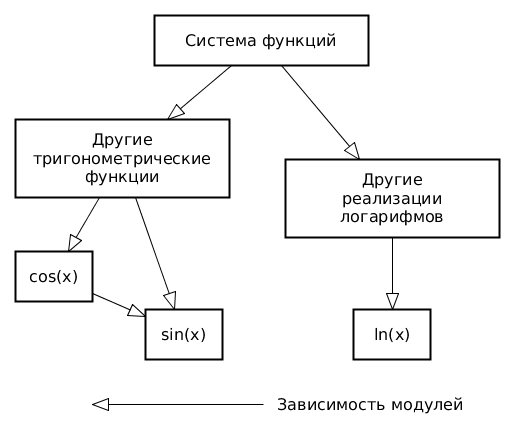
\includegraphics[width=0.5\textwidth]{Lab2_architecture.png}\\
  Рисунок 1. Структура тестируемого приложения
  \end{center}
\item Обе базовые функции ($sin(x)$ и $ln(x)$) должны быть реализованы при помощи разложения в ряд с задаваемой погрешностью. Использовать тригонометрические/логарифмические преобразования для упрощения функций запрещено.
\item Для каждого модуля должны быть реализованы табличные заглушки. При этом необходимо найти область допустимых значений функций и, при необходимости, определить взаимозависимые точки в модулях.
\item Разработанное приложение должно позволять выводить значения, выдаваемое любым модулем системы, в сsv файл вида \verb|X, Результаты модуля (X)|, позволяющее произвольно менять шаг наращивания Х. Разделитель в файле csv можно использовать произвольный.
\end{enumerate}

\section*{UML-диаграмма классов разработанного приложения}

\begin{center}
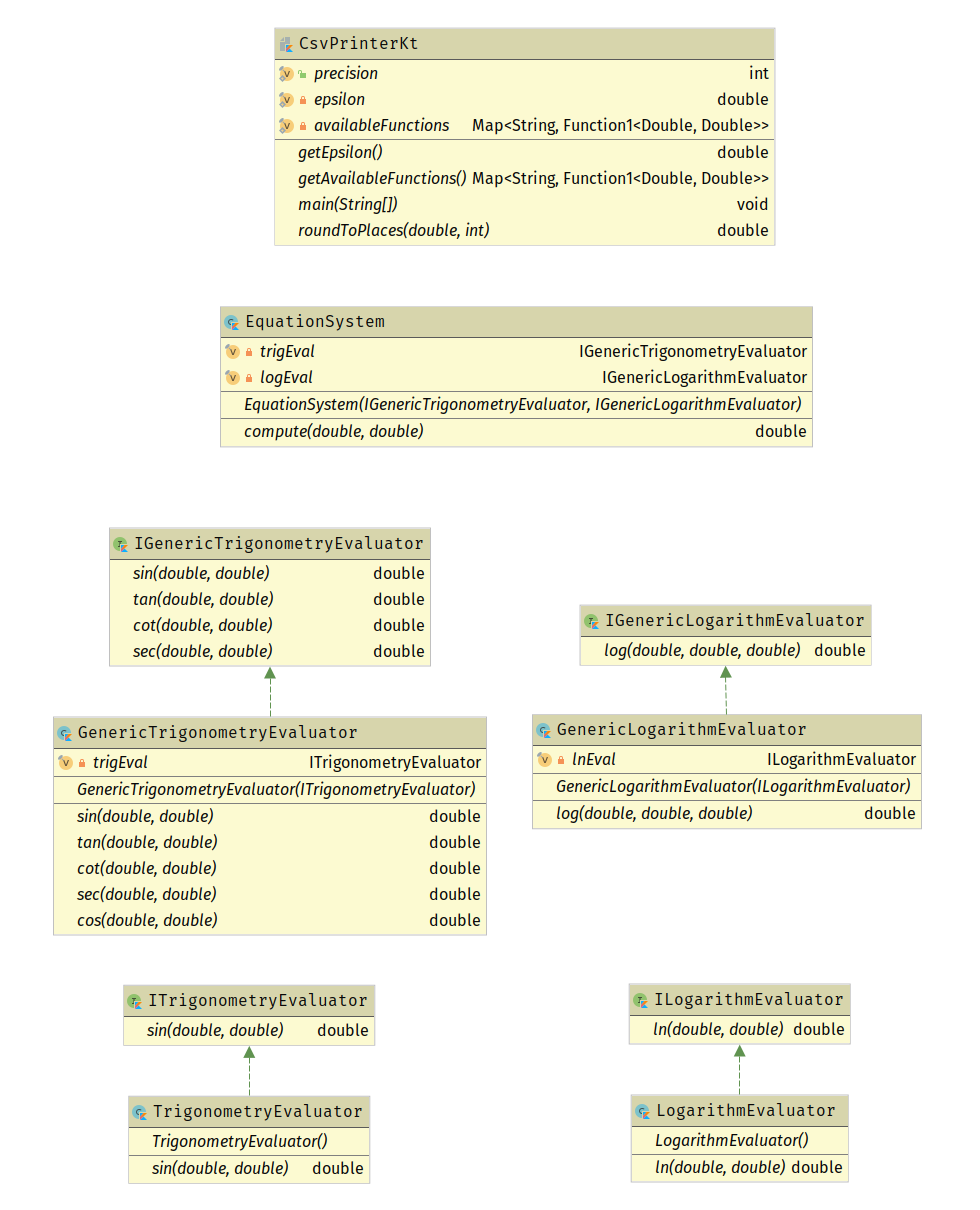
\includegraphics[width=0.9\textwidth]{Lab2_uml.png}\\
Рисунок 2. UML-диаграмма классов разработанного приложения
\end{center}

\newpage
\section*{Описание тестового покрытия}

При разработке была выбрана стратегия интеграции \textit{сверху вниз}. Сначала был реализован модуль
системы функций. Для него были написаны автоматизированные модульные тесты с заглушками тригонометрических
и логарифмических функций. Затем реализован модуль тригонометрических функций и протестирован с заглушкой
модуля аппроксимации синуса, и так далее.

Интеграция приложения производилась по одному модулю, т.е. при наличии нескольких зависимостей создавались
интеграционные тесты для каждой из них по отдельности, и только затем для полной интеграции. Это позволило
быстрее обнаружать ошибки и регрессии: если проблема связана только с одним модулем, то тесты других пройдут,
что явно укажет на источник.

Параллельно разрабатывался модуль вывода значений в CSV файл. Для него была выбрана стратегия интеграции
\textit{end-to-end}, поскольку вывод каждой функции был связан с определенным модулем, и по завершении его
разработки можно было сразу приступать к реализации сценария вывода его результатов.

\section*{Графики функций, используемые в процессе интеграции}

Для тригонометрических функций использовался диапазон значений от $-\frac{7}{6}\pi$ до $\frac{7}{6}\pi$:

\begin{center}
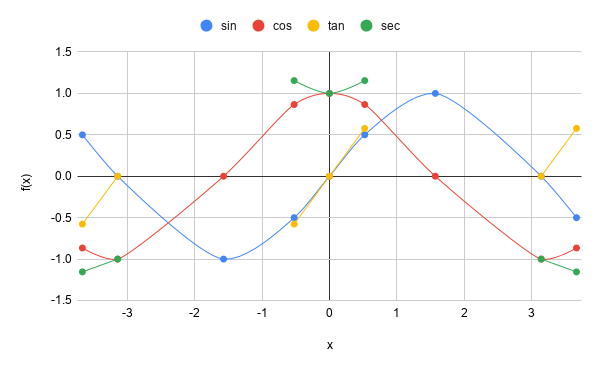
\includegraphics[width=0.9\textwidth]{Lab2_trig_plot.png}\\
Рисунок 3. График тестируемых тригонометрических функций
\end{center}

\newpage
Для логарифма проверялись значения $x < 1$ и $x \geqslant 1$:

\begin{center}
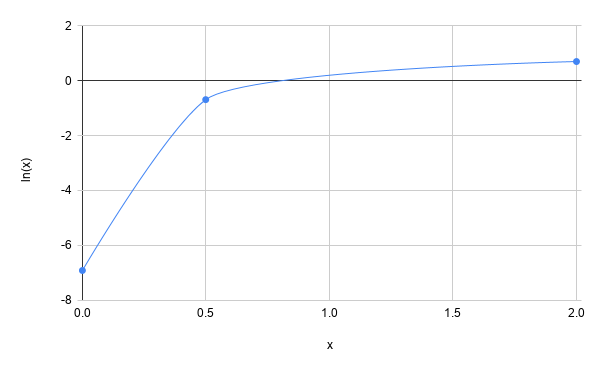
\includegraphics[width=0.9\textwidth]{Lab2_ln_plot.png}\\
Рисунок 4. График тестируемой логарифмической функции
\end{center}

Для системы функций были взяты значения $x < 0$ и $x \geqslant 0$. В левой части
выбирались точки экстремума функции, в правой рассматривались промежутки, где значение
логарифма меньше и больше $0$.

\begin{center}
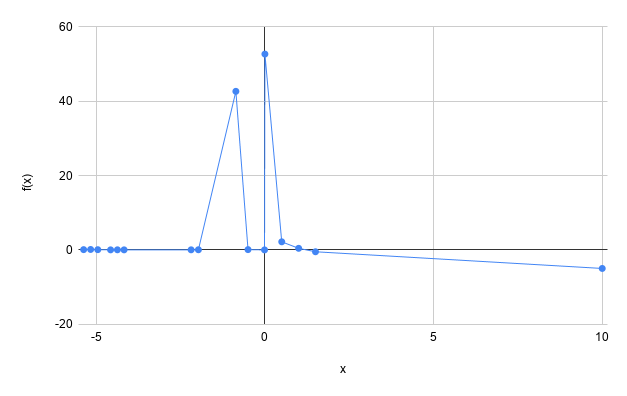
\includegraphics[width=0.9\textwidth]{Lab2_fn_plot.png}\\
Рисунок 5. График тестируемой системы функций
\end{center}

\section*{Исходный код}

\verb|https://github.com/timlathy/itmo-fourth-year/tree/master/Software-Testing-7th-Term/Lab2|

\section*{Выводы}

В ходе выполнения работы было рассмотрено интеграционное тестирование приложения подходом
\textit{сверху вниз} при помощи фреймворка JUnit 5 (модуль Jupiter). При написании
тестов было изучено использование заглушек с применением библиотеки Mockito, а также
загрузка табличных значений для параметризованных тестов из внешних CSV файлов
при помощи аннотации \verb|@CsvFileSource|.

\end{document}
